\documentclass[14pt, a4paper]{article}
\usepackage{extsizes} % Enables ability to change font size
\usepackage{indentfirst}

% Font settings
\usepackage[utf8]{inputenc}
\usepackage[T1,T2A]{fontenc}
\usepackage[russian,english]{babel}
\usepackage{tempora}
\linespread{1.5}

% Indentation settings
\usepackage[a4paper, left=30mm, right=15mm, top=20mm, bottom=20mm]{geometry}

% Paragraph offset size
\setlength\parindent{1.25cm}

% Configure links
\usepackage[spaces,hyphens]{url}
\usepackage[colorlinks,allcolors=black]{hyperref}
\urlstyle{same}

% Configure colors
\usepackage{color}
\definecolor{lightgray}{rgb}{0.9647058823529412,0.9725490196078431,0.9803921568627451}
\definecolor{gray}{rgb}{0.48627450980392156,0.48627450980392156,0.48627450980392156}
\definecolor{blue}{rgb}{0.0,0.3607843137254902,0.7843137254901961}
\definecolor{green}{rgb}{0.27058823529411763,0.49411764705882355,0.2901960784313726}
\definecolor{purple}{rgb}{0.65, 0.12, 0.82}
\definecolor{highlight}{rgb}{0.98, 0.91, 0.71}

% Configure listings
\usepackage{listings}
\lstset{
  basicstyle=\fontsize{12}{13}\ttfamily,
  columns=fullflexible,
  breaklines=true,
  postbreak=\mbox{\textcolor{red}{$\hookrightarrow$}\space},
  escapeinside={\%*}{*)},
  backgroundcolor=\color{lightgray},
  numberstyle=\footnotesize,
  tabsize=2,
  xleftmargin=4ex,
  escapechar=\%
}

% Use style=linesWithNumbers to enable lines enumerating
\lstdefinestyle{linesWithNumbers}{
  numbers=left,
  numberstyle=\color{gray}
}

\lstdefinelanguage{JavaScript}{
  keywords={break, continue, delete, else, for, function, if, in, let, class,
  new, return, this, typeof, var, void, while, with, const, false, null, true, boolean, number, undefined,
  Array, Boolean, Date, Math, Number, String, Object},
  keywordstyle=\color{blue}\bfseries,
  commentstyle=\color{green}\ttfamily,
  stringstyle=\color{purple}\ttfamily,
  sensitive,
  morecomment=[s]{/*}{*/},
  morecomment=[l]//,
  morecomment=[s]{/**}{*/}, % JavaDoc style comments
  morestring=[b]',
  % morestring=[b]",
  morestring=[b]`,
  fontadjust=true,
  showstringspaces=false,
  numbersep=10pt,
}[keywords, comments, strings]

\usepackage{caption}
\usepackage{dirtree} 
\usepackage{graphicx}
\usepackage{float}
\def\code#1{\texttt{#1}} % Inline code

% \setcounter{tocdepth}{4}
% \setcounter{secnumdepth}{4}
\setcounter{page}{4}

\begin{document}
\selectlanguage{russian}

\tableofcontents
\pagebreak

\addcontentsline{toc}{section}{Введение}
\section*{Введение}
Babel $-$ это JavaScript-транскомпилятор, используемый в основном для преобразования кода ECMAScript 
2015+ (ES6+) в более раннюю версию JavaScript. Инструмент применяется для того, чтобы иметь 
возможность использовать все современные возможности языка при разработке и одновременно с этим 
обеспечить совместимость написанного кода со старыми версиями браузеров, не поддерживающими эти новые 
возможности.

Особенностью Babel является его модульная архитектура $-$ трансформации, применяемые к коду, 
описываются в отдельных плагинах, которые можно подключать по отдельности, либо в виде пресета 
(группы плагинов). Также существует возможность создавать свои собственные плагины, чем я и собираюсь
 заняться в рамках выпускной квалификационной работы.

Целью этой работы является создание плагина, позволяющего использовать собственные синтаксические 
конструкции в контексте JavaScript кода. Моя мотивация к выбору этой тематики заключается в желании 
получить более глубокое представление о транспиляции программного кода, а также об устройстве работы 
наиболее популярного из JavaScript транспайлеров $-$ Babel. Кроме того, проделанная работа может 
послужить доказательством концепции (proof of concept), если возникнет желание предложить внесение 
вышеупомянутых собственных синтаксических конструкций в стандарт языка JavaScript.

Данная работа состоит из трех частей. В первой части представлен обзор базовых концепций, 
на которые опирается работа, также приведено описание инструмента Babel и принципов его работы. 
Вторая часть познакомит читателя с API Babel и возможными вариантами его использования. Третья часть 
данной работы содержит описание процесса расширения синтаксиса языка JavaScript в помощью инструмента Babel.

\pagebreak
\section{Базовые концепции}
\subsection{ECMAScript и JavaScript}
ECMAScript $-$ это скриптовый язык программирования общего назначения, стандартизированный международной 
организацией ECMA в спецификации ECMA-262 \cite{ecma-262}. Спецификация ECMA-262 содержит правила и рекомендации, 
которые должны соблюдаться языком программирования, чтобы он считался совместимым с ECMAScript.

ES $-$ сокращение от ECMAScript. Каждая версия языка ECMAScript именуется с помощью сокращения ES и 
номера версии соответственно. Первая версия языка (ES1)  была выпущена в 1997 году. Самое значимое 
обновление язык получил с выходом стандарта версии ES6 (он же ES2015), в котором был добавлен новый 
синтаксис для описания классов, а также поддержка стрелочных функций, констант,  переменных с ограниченной областью 
видимости и так далее.

JavaScript $-$ язык программирования, являющийся реализацией стандарта ECMA-262. Другими словами, 
JavaScript расширяет язык ECMAScript, привнося в него дополнительные возможности.

\subsection{Babel}
Согласно официальной документации \cite{documentation} Babel является JavaScript компилятором. Однако, 
использование термина компилятор здесь не совсем уместно. Обычно под компилятором понимается программа, 
преобразующая исходные тексты программ, написанные на языке программирования высокого уровня, 
непосредственно в машинные инструкции. В большинстве других источников Babel называют транспайлером. 
Транспайлер (или транскомпайлер) $-$ это программа, преобразующая исходный код на одном языке высокого 
уровня в код на другом языке высокого уровня. В случае с Babel $-$ производятся преобразования между 
различными версиями языка JavaScript.

Необходимость в транспилировании JavaScript заключается в желании обеспечить совместимость написанного 
кода с максимальным числом браузеров. Дело в том, что большинство браузеров используют свой отдельный 
JavaScript интерпретатор (в Chrome используется V8, в Firefox $-$ SpiderMonkey, а в Internet Explorer $-$ Chakra), 
и каждый из этих интерпретаторов поддерживает свое независимое подмножество возможностей ES6 (2015). Это 
означает, что код одного и того же приложения может работать для пользователей одних браузеров и не 
работать для пользователей других. Именно эту проблему решает транспиляция кода с помощью Babel. Она 
позволяет использовать современный стандарт JavaScript при разработке и одновременно с этим обеспечить 
широкую поддержку браузеров.

Помимо решения проблемы совместимости, транспайлеры играют важную роль в процессе принятия решений 
комитетом TC39, группой специалистов, ответственных за разработку стандарта ECMAScript. Например, 
Babel поддерживает все экспериментальные возможности языка (находящиеся на рассмотрении комитетом), 
для того чтобы собрать отзывы от реальных пользователей, которые в свою очередь могут повлиять на 
решение членов комитета.


\subsection{Аналоги Babel}
Среди аналогов Babel можно выделить 2 наиболее масштабных, на мой взгляд, проекта: 
\textit{Traceur} и \textit{JSTransform}.

\textit{Traceur} \cite{traceur} - JavaScript транспайлер, предшественник Babel, презентованный компанией Google в 2011 году. 
Ввиду того, что проект перестал поддерживаться разработчиками с 2016 года, Traceur имеет заметно 
меньшую поддержку новых возможностей JavaScript по сравнению с Babel. Также на ограниченную 
функциональность повлиял архитектурный подход, выбранный разработчиками Traceur. Все проводимые над 
кодом трансформации заданы жестко внутри самого транспайлера, что несколько усложняет процесс расширения 
функциональности инструмента. В отличие от монолитной архитектура Traceur, Babel использует систему 
плагинов, с помощью которых описываются трансформации кода. Плагины могут разрабатываться отдельно 
от самого транспайлера и подключаться по востребованию.

\textit{JSTransform} \cite{jstransform} $-$ утилита, разрабатываемая в компании Facebook с 2013 по 2015 год, и изначально используемая 
в процессе сборки проектов на ReactJS. В первую очередь JSTransform позиционировался как
инструмент именно для создания и последующего применения к исходному коду собственных синтаксических преобразований, 
нежели как готовый ES6-to-ES5 транспайлер. По этой причине проект по умолчанию включал лишь небольшой 
набор предопределенных трансформаций. C 2015 проект JSTransform не поддерживается разработчиками и 
не рекомендуется к использованию.

*Здесь юудет вывод по аналогам*

\subsection{Принцип работы Babel}

Транспилирование исходного кода с помощью Babel происходит в три последовательных этапа: парсинг текста 
исходного кода, трансформация и генерация результирующего кода. Прежде чем подробнее рассмотреть каждый из 
этих этапов, необходимо ознакомиться с таким понятием, как \textit{абстрактное синтаксическое дерево}, 
так как оно используется на каждом из трех этапов транспиляции.

\subsubsection{Абстрактное синтаксическое дерево}

Абстрактное синтаксическое дерево (abstract syntax tree, AST) $-$ это древовидное представление структуры исходного кода, написанного
на каком-либо языке программирования. Внутренние узлы такого дерева представляют операторы языка 
программирования, а листья $-$ соответствующие им операнды.  

Дерево называется абстрактным потому, что оно, в отличие от дерева разбора, содержит лишь упрощенную модель программы. При построении
AST игнорируются элементы, не влияющие на семантику исходного кода. Например, в абстрактном синтаксическом
дереве будут отсутствовать группирующие скобки, так как группировка операндов и так явно задана с помощью структуры дерева.

\begin{figure}[h!]
  \centering
  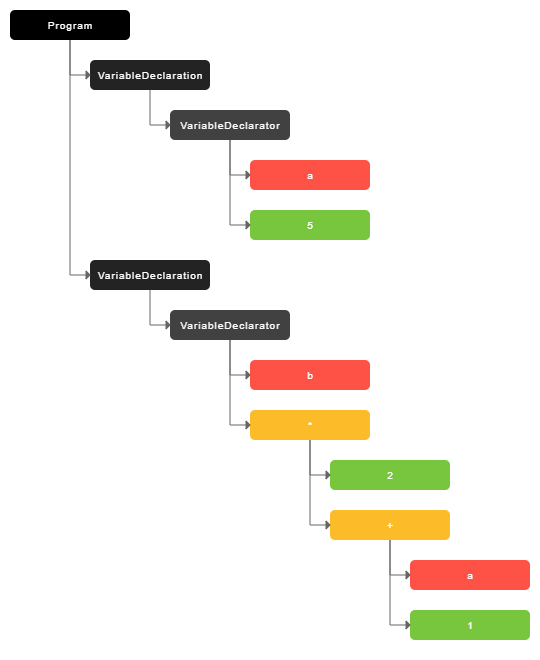
\includegraphics[scale=0.6]{img/ast.png}
  \caption{Пример абстрактного синтаксического дерева}
  \label{ast}
\end{figure}

На рисунке \ref{ast} представлен пример абстрактного синтаксического дерева, построенного для 
следующего фрагмента кода на языка JavaScript:
%  Дерево было построено с использованием парсера,
% входящего в состав транспайлера Babel. 

\lstinputlisting[language=JavaScript, style=linesWithNumbers]{listings/ast-expression.js}

Дерево было построено с использованием парсера, входящего в состав транспайлера Babel.

\subsubsection{Этапы работы Babel}

После того, как было получено представление о понятии AST, можно перейти к обзору основных этапов 
работы Babel, которые представлены на рисунке \ref{babel_stages}.
\begin{figure}[h!]
  \centering
  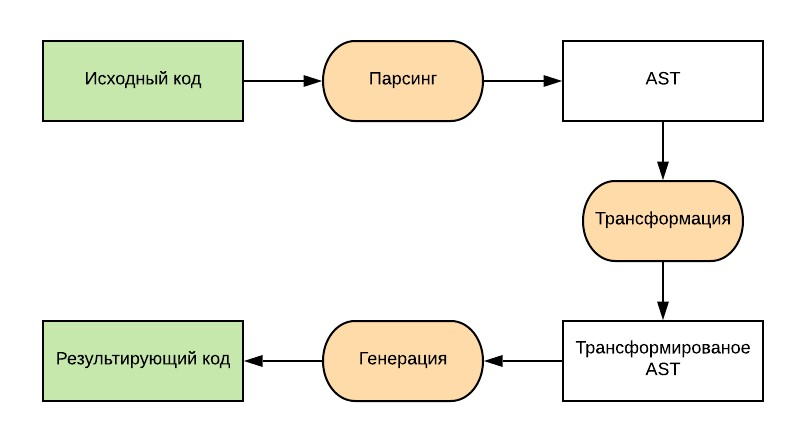
\includegraphics[scale=1.2]{img/babel_stages.jpg}
  \caption{Этапы работы Babel}
  \label{babel_stages}
\end{figure}

\subsubsection*{Парсинг}
На этом этапе код, передаваемый в Babel, конвертируется в абстрактное синтаксическое дерево. 
В свою очередь этап парсинга подразделяется на 
две фазы: \textit{лексический анализ} и \textit{синтаксический анализ}.

В ходе лексического анализа текст исходного кода преобразуется в массив токенов. По этой причине фазу 
лексического анализа часто называют токенизацией. Здесь токен - это объект, описывающий любую значащую 
подпоследовательность символов исходного кода. Например, фрагмент кода

\lstinputlisting[language=JavaScript, style=linesWithNumbers]{listings/fragment-for-tokenization.js}
будет преобразован в следующий массив токенов:

\lstinputlisting[language=JavaScript, style=linesWithNumbers]{listings/tokens.js}
Свойства start и end описывают положение токена в строке, loc $-$ строку, в которой был найден токен. 
Поле type указывает на объект, который хранит набор свойств, описывающих каждый отдельный токен:
\lstinputlisting[language=JavaScript, style=linesWithNumbers]{listings/token-type.js}

Далее следует так называемый синтаксический анализ, цель которого $-$ построение абстрактного 
синтаксического дерева на основе массива токенов, полученного на предыдущем этапе. В ходе этого 
процесса токены преобразуются в узлы дерева (Node), которые кроме уже описанных данных содержат также
информацию о типе узла. Примерами таких типов являются FunctionDeclaration, VariableDeclaration или 
ReturnStatement. Для рассмотренного выше фрагмента кода построенное парсером абстрактное синтаксическое 
дерево будет выглядеть следующим образом:

\lstinputlisting[language=JavaScript, style=linesWithNumbers]{listings/ast-for-fragment.js}

\subsubsection*{Трансформация}
Как только абстрактное синтаксическое дерево построено, начинается этап трансформации. На этом этапе 
производится рекурсивный обход, во время которого добавляются, заменяются или удаляются узлы дерева.
Трансформации, проводимые над деревом, определяются списком подключенных плагинов и применяются в 
порядке их следования в этом списке.

*Используется Посетитель, подробности далее* 

\subsubsection*{Генерация}
По окончании модификации, абстрактное синтаксическое дерево конвертируется обратно в код. 
Происходит это следующим образом: производится обход дерева в глубину, в процессе которого строится строка,
представляющая модифицированный код.

\subsubsection{Шаблон Посетитель}

Обход абстрактного синтаксического дерева, производимый на этапе трансформации, реализован с применением 
шаблона проектирования Посетитель. Это поведенческий шаблон проектирования, впервые описанный в книге 
``Приёмы объектно-ориентированного проектирования. Паттерны проектирования'' \cite{gang_of_4}.
Суть шаблона заключается в предоставлении возможности определять новые операции над объектами,
 не внося изменения в классы этих объектов.

% \subsubsection*{Решаемая проблема}
Проблема, которую решает шаблон Посетитель, можно сформулировать следующим образом:

Необходимо определить ряд несвязанных между собой операций над объектами, принадлежащими определенной структуре.
При этом, требуется избежать модифицирования кода классов этих объектов при добавлении новых операций. 

Шаблон Посетитель описывает решение этой проблемы так:
вместо того чтобы добавлять новое поведение в каждый объект структуры, необходимо вынести это поведение 
в отдельный класс посетителя. Таким образом объекты не будут выполнять операции самостоятельно, а вместо этого 
они будут передаваться в методы посетителя.

Посетитель, в свою очередь, будет содержать множество методов, обрабатывающих объекты разных типов, так как
поведение для них скорее всего будет отличаться. Вопрос, какой именно метод вызывать для каждого конкретного объекта,
разрешается с помощью механизма двойной диспетчеризации. Ответственность за вызов правильного метода посетителя
возлагается на сам объект, передаваемый посетителю в качестве аргумента. Для этого в каждом классе структуры
определяется специальный метод \code{accept(Visitor v)}, внутри которого происходит вызов метода посетителя, соответствующего
типу данного объекта.

На рисунке \ref{visitor_uml} представлена UML диаграмма, иллюстрирующая классическую реализацию шаблона
Посетитель. Диаграмма состорит из следующих компонентов:
\begin{itemize}
  \item \textbf{Visitor} $-$ описывает общий интерфейс для всех посетителей. Содержит объявления 
    методов \code{visit} для каждого конкретного типа элементов. 
  \item \textbf{ConcreteVisitor} $-$ конкретный класс посетителя, реализует интерфейс, определенный в Visitor.
  \item \textbf{Element} $-$ интерфейс, содержащий объявление метода \code{accept}.
  \item \textbf{ElementA / ElementB} $-$ конкретные классы элементов структуры, реализуют метод \code{accept}
    интерфейса Element, вызывая внутри него метод Посетителя, соответствующий своему типу.
  \item \textbf{Client} $-$ класс-пользователь структуры объектов. В нем происходит вызов метода \code{accept}
    объекта с конкретным экземпляром Посетителя.
\end{itemize}

\begin{figure}[h!]
  \centering
  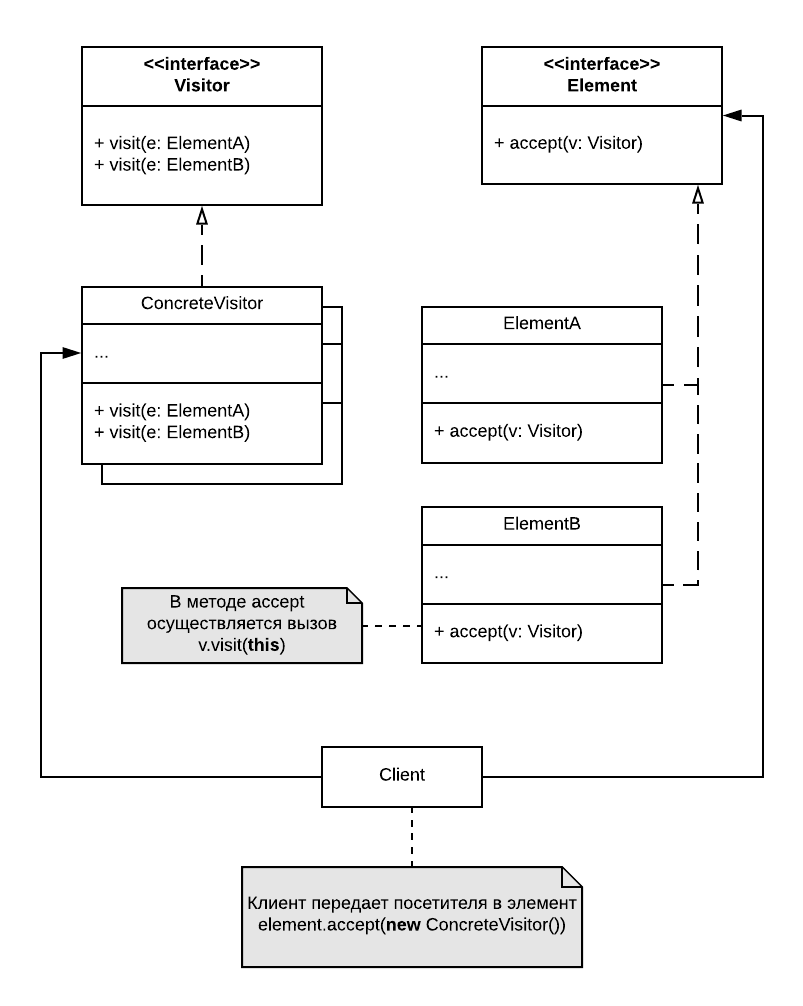
\includegraphics[scale=1.0]{img/visitor_uml.png}
  \caption{UML диаграмма компонентов шаблона Посетитель}
  \label{visitor_uml}
\end{figure}

Шаблон Посетитель широко используется в реализация различных компиляторов для определения операций над 
абстрактными синтаксическими деревьями. Babel, компилирующий JavaScript код в другой JavaScript код,
также не является исключением. Однако, из-за ограничений языка программирования JavaScript, таких как
отсутствие поддержки перегрузки методов и возможности определять интерфейсы, реализация шаблона Посетитель
в Babel несколько отличается от классической.

В Babel посетить представляет из себя обычный JavaScript объект, который содержит методы, чьи названия 
совпадают с типом узлов AST, которые они ``посещяют''.

\lstinputlisting[language=JavaScript, style=linesWithNumbers]{listings/visitor_expample.js}

Внутри методов Посетителя определяются операции, которые необходимо произвести над узлами данного типа.
Узлы абстрактного синтаксического дерева в Babel не содержат метода \code{accept}. Вместо этого за вызов
подходящего метода Посетителя отвечает функция \code{traverse}, выполняющая обход дерева. Ниже приведен 
псевдокод, упрощенно иллюстрирующий механизм работы этой функции.

\lstinputlisting[language=JavaScript, style=linesWithNumbers]{listings/traverse.js}

 *Написать, что плагины Babel используют шаблон посетитель, чтобы описывать трансформации синтаксических деревьев*

\pagebreak

\section{Babel API}

*Описать пакеты @babel/core, @babel/cli, @babel/parser, @babel/traverse, @babel/generator, @babel/plugin и варианты их использования* 
 

\pagebreak

\section{Расширение синтаксиса языка JavaScript с помощью Babel}
% В данной главе описан процесс создания плагина для транспайлера Babel. В качестве 
\subsection{Постановка задачи}
Необходимо расширить функциональность транспайлера Babel таким, чтобы с его помощью можно было использовать 
синтаксическую конструкцию \code{deep spread} оператор в рамках JavaScript кода. 

Идея нового \code{deep spread} оператора заключается в улучшении существующего в языке JavaScript обычного \code{spread}
оператора. По этой причине требуется сначала ознакомиться с работой существующего оператора для лучшего понимания вопроса.

\subsubsection{Обычный spread оператор}
% Spread оператор позволяет переписать элементы итерируемых объектов в новый целевой объект. 
Spread оператор (или оператор расширения)\cite{spread_mozilla} позволяет расширить итерируемые объекты и положить их 
содержимое в индивидуальные элементы. Оператор имеет синтаксис \code{...arg}, где 
\code{arg} может быть представлен объектом, массивом или строкой. Спецификация языка допускает следующие 
варианты использования этого оператора:
\begin{itemize}
  \item {Для функций. Позволяет отобразить элементы массива на аргументы функции при ее вызове.}
  \lstinputlisting[language=JavaScript, style=linesWithNumbers]{listings/spread-expample-func.js}
  \item {Для литералов массивов и строк. Позволяет использовать элементы массивов в качестве отдельных значений.}
  \lstinputlisting[language=JavaScript, style=linesWithNumbers]{listings/spread-example-array.js}
  \item {Для литералов объектов. Позволяет использовать пары ключ-значение исходного объекта в качестве отдельных значений.}
  \lstinputlisting[language=JavaScript, style=linesWithNumbers]{listings/spread-example-obj.js}
\end{itemize}
Важно отметить, что при использовании \code{spread} оператора создается копия элементов 
итерируемого объекта, к которому применяется оператор. По этой причине наиболее частым вариантом 
использования данного оператора является копирование массивов или объектов. В следующем фрагменте 
кода приведен пример создания копии объекта с использованием \code{spread} оператора:
\lstinputlisting[language=JavaScript, style=linesWithNumbers]{listings/copy-obj-with-spread.js}
Однако стоит обратить внимание на тот факт, что при копировании с использованием \code{spread} оператора
создается лишь неглубокая копия исходного объекта. Это означает, что при наличии вложенных структур, 
они будут скопированы по ссылке. 

\subsubsection{Deep spread оператор}
Deep spread оператор (или глубокий оператор расширения) $-$ это не существующий в стандарте языка ECMAScript оператор, поддержку которого 
планируется осуществить средствами транспайлера Babel в рамках данной выпускной квалификационной работы.

По задумке \code{deep spread} оператор должен повторять возможности обычного \code{spread} оператора с тем отличием,
что будет всегда создавать глубокие (рекурсивные) копии операндов. Новый оператор будет иметь синтаксис \code{...\#arg},
где \code{arg} может быть представлен объектом или массивом. Ниже приведен пример потенциального 
использования подобного оператора.
\lstinputlisting[language=JavaScript, style=linesWithNumbers]{listings/copy-with-deep-spread.js}

\subsection{План работ}
Для того чтобы добавить поддержку новой синтаксической конструкции \code{deep spread} оператор в 
транспайлер Babel, потребуется выполнить следующую последовательность шагов:
\begin{enumerate}
  \item Расширить парсер Babel, добавив в него возможность корректно распознавать последовательность символов 
    ``\code{...\#}''. 
  \item Написать плагин для Babel, позволяющий трансформировать код, содержащий \code{deep spread} оператор,
  в валидный JavaScript код.
  
  % Трансформация будет происходить следующим образом: операнды всех \code{spread} операторов
  % с флагом \code{deep = true} будут обернуты в вызов функции, возвращающей рекурсивную копию аргумента.
  % Определение самой функции будет добавляться в глобальную область видимости во время транспиляции. 
\end{enumerate}

\subsection{Используемые инструменты}
\begin{itemize}
  \item \textit{git} $-$ распределенная система контроля версий для отслеживания изменений в исходном коде 
    во время разработки программного обеспечения.
  \item \textit{GitHub} $-$ крупнейший веб-сервис для хостинга git репозиториев.
  \item \textit{make} $-$ инструмент для автоматизации сборки программных проектов. Конфигурируется с помощью файла 
    \code{Makefile}.
  \item \textit{NodeJS} $-$ кроссплатформенная среда выполнения JavaScript c открытым исходным кодом.
    Основана на движке \code{V8}. Позволяет выполнять JavaScript код за пределами веб-браузера.
  \item \textit{npm} $-$ пакетный менеджер, входящий в состав NodeJS.
  \item \textit{AST Explorer} $-$ инструмент, упрощающий процесс исследования абстрактных 
    синтаксических деревьев, построенных с применением различных парсеров.
\end{itemize}


\subsection{Процесс реализации}
\addcontentsline{toc}{subsubsection}{Шаг 1. Расширение парсера Babel}
\subsubsection*{Шаг 1. Расширение парсера Babel}
Согласно составленному плану работ первым делом необходимо расширить возможности транспайлера Babel таким образом,
чтобы он смог корректно распознавать новый синтаксис. Для этого следует сделать форк репозитория Babel,
расположенного на сервисе GitHub по адресу \url{https://github.com/babel/babel}. Создание форка - это
получение собственной копии чужого проекта с целью внести изменения или исправления ошибок. При желании
из скопированного с помощью форка репозитория можно сделать Pull Request в оригинальный репозиторий,
таким образом предложив внести свои изменения в основной проект.
\begin{figure}[h!]
  \centering
  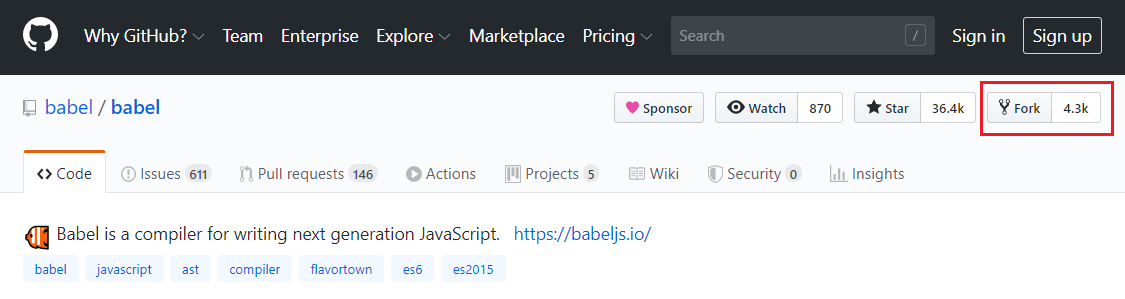
\includegraphics[scale=0.55]{img/babel_fork.PNG}
  \caption{Создание форка проекта Babel}
  \label{babel_fork}
\end{figure}

После того как сделан форк проекта, следует получить локальную копию репозитория проекта, выполнив следующую команду:
\begin{lstlisting}
 > git clone https://github.com/{github_name}/babel.git
\end{lstlisting}

Далее нужно создать новую ветку, которая будет содержать все изменения, касающиеся добавления поддержки нового оператора.
Сделать это можно, выполнив следующую команду:
\begin{lstlisting}
  > git checkout -b deep-spread-operator
\end{lstlisting}

% Для автоматизации задач в проекте Babel используется утилита \code{make}, конфигурируемая файлом 
% \code{Makefile}. Первым шагом будет установка зависимостей путем исполнения следующей команды в 
% корневой директории проекта:

% \begin{lstlisting}
%   > make bootstrap
% \end{lstlisting}

Первым шагом будет установка зависимостей проекта. Сделать это можно, вызвав утилиту \code{make} и передав 
в качестве параметра название задачи по установке зависимостей $-$ \code{bootstrap}. Сам сценарий задачи 
описан в файле \code{Makefile}.

\begin{lstlisting}
  > make bootstrap
\end{lstlisting}

Проект организован в виде монорепозитория. Это означает, что код множества независимых подпроектов,
таких как babel-parser или babel-cli, хранится в одном git репозитории. Структура репозитория Babel
представлена на рисунке \ref{babel_dirs}.

\begin{figure}[H]
\centering
\framebox[\textwidth]{%
\begin{minipage}{0.9\textwidth}
  \dirtree{%
    .1 babel.
    .2 packages.
    .3 babel-cli.
    .3 babel-parser.
    .3 babel-plugin-transform-classes.
    .3 babel-traverse.
    .3 \ldots .
    .2 Gulpfile.js.
    .2 Makefile.
    .2 package.json.
    .2 \ldots.
  }
\end{minipage}
}
\caption{Структура репозитория Babel}
\label{babel_dirs}
\end{figure}


Независимые пакеты, входящие в состав Babel, находятся в директории \code{packages/}. Для того, чтобы 
расширить парсер, необходимо внести изменения в пакет \code{babel-parser}.

\textit{Примечание.} Исходный код проекта Babel напиcан на языке программирования JavaScript с 
применением синтаксического анализатора Flow. Этот инструмент позволяет выполнять проверку типов во 
время компиляции. По желанию можно также использовать аннотации типов в рамках JavScript кода, которые
будут удалены во время сборки проекта. Файлы, в которых производится проверка типов с применением Flow,
начинаются со служебного комментария \code{//@flow}.

\paragraph{Добавление поддержки нового типа токена} \mbox{}\\

Первым делом следует ``научить'' токенизатор Babel распознавать последовательность символов ``\code{...\#}'' 
как самостоятельный токен. Все поддерживаемые при парсинге токены перечислены в экспортируемом объекте 
\code{types} в файле \code{babel/packages/babel-parser/src/tokenizer/types.js}. Чтобы включить поддержку нового токена,
следует добавить новое поле в объект \code{types}. Название поля должно соответствовать имени токена, в данном случае это \code{ellipsisHash}.
В качестве значения следует указать результат вызова функции-конструктора нового токена с оператором \code{new}. 

\lstinputlisting[language=JavaScript, style=linesWithNumbers, caption={Добавление токена ellipsisAt}]{listings/add-new-token.js}

Далее требуется внести изменения в сам токенизатор Babel таким образом, чтобы при появлении последовательностей символов 
``\code{...\#}'' в тексте исходного кода создавался объявленный ранее токен \code{ellipsisHash}. Для этого 
потребуется внести изменения в файл \code{babel/packages/babel-parser
/src/tokenizer/index.js}, а именно добавить дополнительное условие в метод \code{readToken\_dot()} класса \code{Tokenizer}, отвечающий за распознавание токенов,
содержащих символ ``.'' (точка).
\lstinputlisting[language=JavaScript, style=linesWithNumbers, label={readTokenDot}, caption=Метод readToken\_dot() класса Tokenizer]{listings/add-condition-to-tokenizer.js}

На листинге \ref{readTokenDot} выделены строки кода, добавленные для того, чтобы токенизатор Babel 
получил способность корректно распознавать описанную выше последовательность символов. В них происходит 
проверка на факт наличия символа ``\#'' за тремя подряд идущими символами ``.'' (точка).
Если такой символ найден, то создается токен \code{ellipsisHash}, в противном случае
$-$ простой \code{ellispis} (с английского $-$ многоточие).

\paragraph{Изменение AST} \mbox{}\\

После того как в токенизатор Babel была добавлена возможность распознавать токен \code{ellipsisHash},
следует также внести изменения в сам парсер. Чтобы понять, какие именно требуются изменения, можно посмотреть на то, какое
синтаксическое дерево строится для выражения, содержащего обычный \code{spread} оператор. Для этого удобно использовать 
инструмент AST Explorer (\url{https://astexplorer.net}), в котором следует язык JavaScript и парсер babel-v7.
В левую панель инструмента вводится исходный код на выбранном языка программирования, после чего на 
правой панели отображается результат парсинга введенного кода с помощью выбранного парсера.

В данном случае в качестве исходного кода вводится строка, содержащая \code{spread} оператор, например
\code{const a = \{...\{c: 1\}\}}. Если навести курсор на рассматриваемый оператор, то соответствующий 
ему узел синтаксического дерева подсветится на панели справа. Как видно на рисунке \ref{ast_explorer},
в данному случае узел имеет тип \code{SpreadElement}.

\begin{figure}[h!]
  \centering
  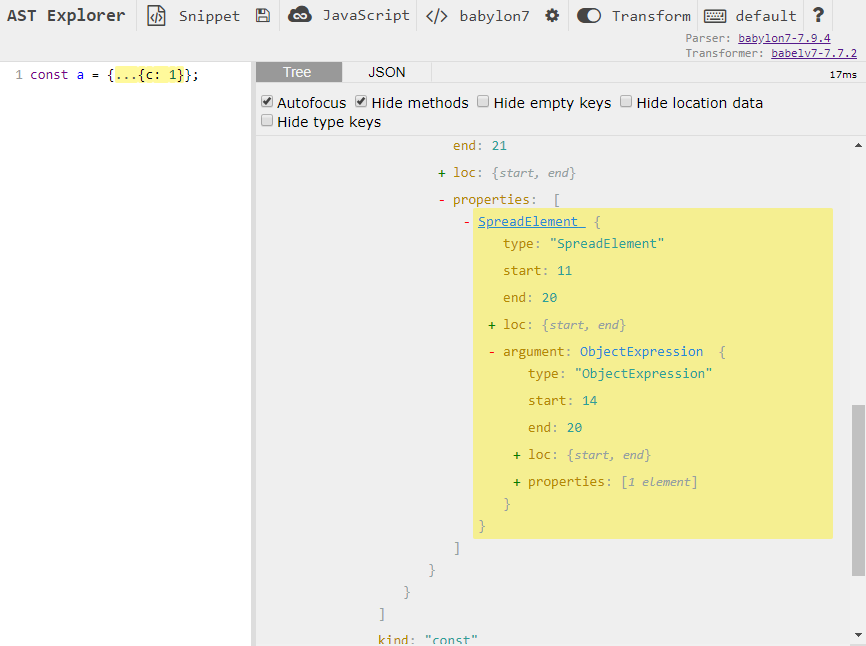
\includegraphics[scale=0.7]{img/ast-explorer.png}
  \caption{Исследование синтаксического дерева выражения с помощью AST Explorer}
  \label{ast_explorer}
\end{figure}

После того как стало известно, какой тип узла синтаксического дерева соответствует обычному \code{spread}
оператору, требуется расширить этот тип, добавив в него новый атрибут \code{deep: boolean}. Новый атрибут
нужен для того чтобы отличать между собой два вида \code{spread} операторов: глубокий и обычный. 
В листинге \ref{addDeepAttr} представлены изменения, внесенные в файл \code{babel/packages/babel-parser/src/types.js}


%  Далее необходимо расширить найденный тип узла \code{SpreadElement}, добавив в него новый атрибут \code{deep: boolean}

% Добавим новый атрибут \code{deep: boolean} в тип узла \code{SpreadElement}. Новый атрибут будет указывать,
% должен ли \code{spread} оператор возвращать рекурсивную копию операнда $-$ в случае с \code{deep spread} оператором,
% или нет $-$ в случае с обычным \code{spread} оператором. Так как все типы узлов синтаксического дерева 
% определены в файле \code{babel/packages/babel-parser/src/types.js}, именно в него и нужно внести изменения. 

\lstinputlisting[language=JavaScript, style=linesWithNumbers, label={addDeepAttr}, caption={Добавление атрибута deep в тип узла SpreadElement}]{listings/add-deep-attr.js}
% Первым делом добавим новый атрибут \code{deep: boolean}
% в тип \code{SpreadElement}, описывающий соответствующий узел абстрактного синтаксического дерева (листинг \ref{addDeepAttr}).
% Все типы узлов дерева определены в файле \code{babel/packages/
% babel-parser/src/types.js}


% Посмотрим на обычный SpreadExpression через AST explorer 
Для того чтобы новый атрибут корректно инициализировался, требуется также изменить метод \code{parseSpread} класса
\code{LValParser}, объявленного в файле \code{babel/packages/babel-parser/src/parser/lval.js} (листинг \ref{parseSpread}). 
В метод следует добавить новый аргумент \code{isDeep: boolean} со значением \code{false} по умолчанию.
Значением этого аргумента будет инициализироваться поле \code{deep} создаваемого узла.

\lstinputlisting[language=JavaScript, style=linesWithNumbers, label={parseSpread}, caption={Добавление аргумента isDeep в метод parseSpread класса LValParser}]{listings/parse-spread.js}

% Далее следует обновить места вызовов этого метода.
Далее следует обновить участки кода, в которых происходит вызов метода \code{parseSpread}. Для этого
необходимо внести изменения в методы \code{parseObjectMember} и \code{parseExprListItem} класса \code{ExpressionParser},
объявленного в файле \code{babel/packages/babel-parser/src/parser/expression.js}.
С подробным листингом внесенных изменений можно ознакомиться в приложении.


\addcontentsline{toc}{subsubsection}{Шаг 2. Создание плагина для Babel}
\subsubsection*{Шаг 2. Создание плагина для Babel}
После того как в парсер Babel были внесены необходимые изменения, можно приступить к созданию плагина,
с помощью которого будет проводиться трансформация нового синтаксиса в валидный JavaScript код.

Для этого в директории \code{babel/packages} необходимо создать новую директорию \code{babel-plugin-transform-deep-spread-operator}.
Далее следует перейти в созданную директорию и выполнить команду \code{npm init}, которая создаст
файл \code{package.json}. Файл \code{package.json} является дескриптором NodeJS модуля и необходим 
для того, чтобы модуль можно было устанавливать как зависимость в других проектах с помощью пакетного
менеджера npm. После этого требуется создать файл \code{src/index.js}, который непосредственно будет 
содержать исходный код плагина. Полученная структура директории плагина представлена на рисунке \ref{babel_plugin_dirs}.

% \begin{figure}[H]
%   \centering
%   \framebox[\textwidth]{%
%   \begin{minipage}{0.9\textwidth}
%     \dirtree{%
%       .1 babel-plugin-transform-deep-spread-operator.
%       .2 lib.
%       .3 index.js.
%       .2 node\_modules.
%       .2 src.
%       .3 index.js.
%       .2 package.json.
%     }
%   \end{minipage}
%   }
%   \caption{Структура директории плагина}
%   \label{babel_plugin_dirs}
% \end{figure}


\begin{figure}[H]
  \centering
  \framebox[\textwidth]{%
  \begin{minipage}{0.9\textwidth}
    \dirtree{%
      .1 babel.
      .2 packages.
      .3 \ldots .
      .3 babel-plugin-transform-deep-spread-operator.
      .4 lib.
      .5 index.js.
      .4 node\_modules.
      .4 src.
      .5 index.js.
      .4 package.json.
      .2 \ldots.
    }
  \end{minipage}
  }
  \caption{Структура директории плагина}
  \label{babel_plugin_dirs}
  \end{figure}

Листинг \ref{plugin} содержит исходный код плагина. Ключевыми здесь являются строки 9-19, в которых определен 
объект \code{visitor}. Внутри этого объекта определена функция \code{SpreadElement}, в которой описываются
действия, которые необходимо произвести над узлами синтаксического дерева транспилируемой программы, 
тип которых соответствует названию функции. Такая конструкция является элементом паттерна Посетитель, с которым 
можно ознакомиться более подробно в первой главе данной работы. В данном случае в функции \code{SpreadElement}
проверяется условие наличия у текущего узла флага \code{deep = true}. Если условие выполняется, то 
производится замена значения свойства \code{argument} текущего узла на вызов вспомогательной функции \code{deepCopy} 
с прежним значением свойства \code{argument} в качестве параметра. 
Функция \code{deepCopy} возвращает рекурсивную копию передаваемых в нее объектов.

\lstinputlisting[language=JavaScript, style=linesWithNumbers, label={plugin}, caption={Плагин Babel}]{listings/plugin/plugin.js}

% Для того чтобы вспомогательная функция \code{deepCopy} была доступна на момент вызова, следует добавить ее определение в 
% пакет \code{@babel/helpers}. В этом пакете объявляются всевозможные функции, которые используются многими 
% плагинами в ходе трансформаций исходного кода. 

Для того чтобы вспомогательная функция \code{deepCopy} была доступна на момент вызова, ее следует 
добавлять в глобальную область видимости исходной программы во время транспиляции. Легче всего это можно сделать,
добавив ее определение в пакет \code{@babel/helpers}. В этом пакете объявляются всевозможные функции,
которые используются многими плагинами в ходе трансформаций исходного кода.

% добавить ее определение в 
% пакет \code{@babel/helpers}. В этом пакете объявляются всевозможные функции, которые используются многими 
% плагинами в ходе трансформаций исходного кода.


\lstinputlisting[language=JavaScript, style=linesWithNumbers, label={helper}, caption={Объявление вспомогательной функции}]{listings/plugin/helper.js}

После того как сделаны необходимые изменения, требуется произвести сборку проекта с помощью команды
\begin{lstlisting}
  > make build
 \end{lstlisting}

Далее можно закрепить изменения в \code{git} репозитории данного проекта, выполнив следующую последовательность команд:
\begin{lstlisting}
  > git add .
  > git commit -m "Add support of deep spread operator to babel-parser"
\end{lstlisting}

Последним шагом будет отправка сделанных изменений в собственный удаленный репозиторий на GitHub (который
в свою очередь является форком оригинального репозитория Babel)
\begin{lstlisting}
  > git push --set-upstream origin deep-spread-operator
\end{lstlisting}
\subsection{Демонстрация результатов}

Для проверки результатов проделанной работы потребуется создать тестовый проект. Структура тестового проекта 
представлена на рис \ref{test_struct}.
\begin{figure}[h!]
  \centering
  \framebox[\textwidth]{%
  \begin{minipage}{0.9\textwidth}
    \dirtree{%
      .1 test.
      .2 node\_modules.
      .2 out.
      .3 index.js.
      .2 src.
      .3 out.js.
      .2 babel.config.json.
      .2 package.json.
    }
  \end{minipage}
  }
  \caption{Структура директории плагина}
  \label{test_struct}
\end{figure}

% В файле \code{package.json} в качестве зависимостей следует указать @babel/cli, @babel/core и 
% @babel/plugin-transform-deep-spread-operator. Для двух последних пакетов вместо версии 
% следует указать путь к месторасположению собранного пакета в файловой системе. Таким образом 
% зависимости не будут скачиваться из реестра npm, вместо этого будут использоваться локально расположенные 
% файлы.

В файле \code{package.json} в качестве зависимостей следует указать @babel/cli, @babel/core и 
@babel/plugin-transform-deep-spread-operator. Для двух последних пакетов вместо версии 
следует указать путь к месторасположению собранного пакета в файловой системе. Таким образом вместо 
того чтобы скачивать зависимости из удаленного реестра, npm будет брать локально расположенные файлы.
В данном случае это необходимо, поскольку локальные пакеты содержат изменения, обеспечивающие поддержку 
нового оператора.

\lstinputlisting[language=JavaScript, style=linesWithNumbers, label={package}, caption={Файл package.json}]{listings/test/package.json}
Далее следует произвести установку зависимостей, выполнив команду
\begin{lstlisting}
  > npm install
\end{lstlisting}

С помощью файла \code{babel.config.json} задается конфигурация Babel. В данном случае задан только 
список подключенных плагинов, содержащий один элемент $-$ \code{plugin-transform-deep-spread-operator}.

\lstinputlisting[language=JavaScript, style=linesWithNumbers, label={package}, caption={Файл babel.config.json}]{listings/test/babel.config.json}


В файл \code{src/index.js} (листинг \ref{src}) поместим исходный код на языке JavaScript, содержащий 
использование нового \code{deep spread} оператора.

\lstinputlisting[language=JavaScript, style=linesWithNumbers, label={src}, caption={Код до транспиляции}]{listings/test/src.js}

Далее в корневой директории данного Тестового проекта выполним команду \code{npm run babel}

\begin{figure}[H]
  \centering
  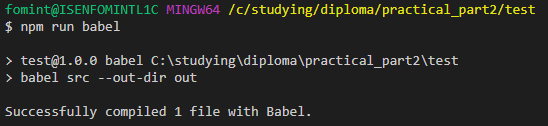
\includegraphics[scale=1.0]{img/test_run_babel.PNG}
  \caption{Запуск транспиляции}
  \label{test_run_babel}
\end{figure}

Выполнение этой команды запустит скрипт с названием \code{babel}, описанный в 7 строке файла 
\code{package.json}. Этот скрипт произведет транспиляцию файла \code{src/index.js} с помощью Babel и 
запишет результат в файл \code{out/index.js}. 

\lstinputlisting[language=JavaScript, style=linesWithNumbers, label={out}, caption={Код после транспиляции}]{listings/test/trgt.js}

Листинг \ref{out} содержит код, полученный в результате транспиляции. Можно заметить, что в глобальную
область видимости была добавлена функция рекурсивного копирования \code{\_deepCopy} (строка 1). 
Далее была произведена замена \code{deep spread} оператора на обычный \code{spread} оператор, операнд
которого был обернут в функцию \code{\_deepCopy} (строка 9). 

Проверим, действительно ли с помощью подобной замены получается рекурсивная копия объекта. Для этого
исполним полученный в ходе транспиляции файл \code{out/index.js} с помошью NodeJS:

\begin{figure}[H]
  \centering
  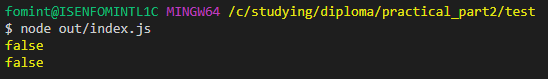
\includegraphics[scale=1.0]{img/test_results.PNG}
  \caption{Проверка результатов транспиляции}
  \label{test_results}
\end{figure}
Как можно увидеть на рисунке \ref{test_results}, при выполнении файла в терминал выводится значение 
\code{false} два раза. Первый \code{false} $-$ это результат сравнения ссылок на исходный и 
скопированный объекты (строка 11 файла \code{out/index.js}). Второй \code{false} $-$ результат сравнения
вложенных объектов (строка 13 файла \code{out/index.js}). Таким образом, мы получили рекурсивную копию
объекта. 


\pagebreak
\section{Заключение}
\pagebreak

\addcontentsline{toc}{section}{Список литературы}
\begin{thebibliography}{9}
  \bibitem{ecma-262} Стандарт ECMA-262 [Электронный ресурс] $-$ Режим доступа: \linebreak
    \url{https://www.ecma-international.org/publications/standards/Ecma-262.htm}
  \bibitem{documentation} Документация Babel [Электронный ресурс] $-$ Режим доступа: \linebreak
    \url{https://babeljs.io/docs/en}
  \bibitem{traceur} Документация Traceur [Электронный ресурс] $-$ Режим доступа: \linebreak
    \url{https://github.com/google/traceur-compiler/wiki/Getting-Started}
  \bibitem{jstransform} Репозиторий JSTransform на сервисе GitHub [Электронный ресурс] $-$ Режим доступа:
    \url{https://github.com/facebookarchive/jstransform}
  \bibitem{gang_of_4} Э. Гамма, Р. Хелм, Р. Джонсон, Д. Влиссидес. Приёмы объектно-ориентированного проектирования. Паттерны проектирования, СПб.: Питер, 2017. $-$ 368 с.: ил.
  \bibitem{spread_mozilla} Описание spread синтаксиса на ресурсе MDN web docs [Электронный ресурс] $-$ Режим доступа:
    \url{https://developer.mozilla.org/en-US/docs/Web/JavaScript/Reference/Operators/Spread_syntax}
\end{thebibliography}

\pagebreak
\addcontentsline{toc}{section}{Приложение}
\section*{Приложение}
\lstinputlisting[language=JavaScript, style=linesWithNumbers, label={parseCall}, caption={Добавление аргумента isDeep в метод parseSpread класса LValParser}]{listings/parse-object-member.js}

\end{document}

